% !TeX root = ../main.tex
% Add the above to each chapter to make compiling the PDF easier in some editors.

\chapter{Testing}\label{chap:testing}

In this chapter, we will be discussing the way we tested our prototype
implementation and the results we obtained from these tests.
We will mainly consider basic metrics such as delay reduction and 
CPU utilization to make sure the fundamental impact of our prototype
is analyzed.
Further testing might be especially interesting after the integration
of a working congestion handling mechanism into our prototype.

\section{Setups}\label{sec:setups}

We test the performance of our prototype in a lab-like environment that 
allows us to maintain a stable network state.
We do this by using Linux network namespaces where each namespace represents
a different participant in the communication, i.e.~the server, the relay, and the client.
A schematic overview of the setup is shown in \autoref{fig:namespace-setup}.

% \vspace{0.5cm}
% \begin{figure}[H]
% \centering
% \begin{myverbatim}
        
%                                     interface: veth1                      interface: veth3
%                                     ip: 192.168.1.2/24                    ip: 192.168.1.4/24
%               interface: veth0       \              interface: veth2       \
%               ip: 192.168.1.1/24      \             ip: 192.168.1.3/24      \
%  __________  /                         \  _______  /                         \  __________ 
% |          |/                           \|       |/                           \|          |
% |  Server  |-------> veth0@veth1 ------->| Relay |-------> veth2@veth3 ------->|  Client  |
% |__________|<------- veth1@veth0 <-------|_______|<------- veth3@veth2 <-------|__________|
        
% \end{myverbatim}
% \caption{Logical setup including interfaces and IPs}\label{fig:logical-setup}
% \end{figure}
% \vspace{0.5cm}

\vspace{0.5cm}
\begin{figure}[H]
\centering
\begin{myverbatim}
 ______________________         _______________________________________        ______________________
|   Server namespace   |       |            Relay namespace            |      |   Client namespace   |
|     ____________     |       |    ______________   ______________    |      |     ____________     |
|    |192.168.10.1|    |       |   | 192.168.10.2 | | 192.168.11.2 |   |      |    |192.168.11.1|    |
|____|___veth0____|____|       |___|____veth1_____|_|____veth2_____|___|      |____|____veth3___|____|
            \                            /                 \                             /
             \                          /                   \                           /
              \                        /                     \                         /
               \                      /                       \                       /
                \ __________________ /_                      __\ ___________________ /
                /veth0-br|     |veth1-br\                   /veth2-br|      |veth3-br\
                |                    ___|                   |___                     |
                \_____v-net-0_______|NAT/                   \NAT|_________v-net-1____/
                        /              \                     /                \
               ip: 192.168.10.10        \                   /         ip: 192.168.11.10
               net: 192.168.10.0/24      \   ___________   /          net: 192.168.11.0/24
                                           /             \
                                          |   enp1s0f0    |
                                           \ ___________ /
                                                  |
                                                  |
                                              (INTERNET)

\end{myverbatim}
\caption{Local setup including bridges and namespaces}\label{fig:namespace-setup}
\end{figure}
\vspace{0.5cm}

\subsection{Local Environment for Testing and Development}\label{subsec:namespace_environment}
The local environment we use for testing and developing allows us to setup the network in a way 
that fits the current needs of the prototype.
One example for such needs would be that we need a slight delay between sending a packet and 
receiving its acknowledgment since the registering of a sent packet takes place after a packet 
is sent out. 
In a real-world scenario this would obviously also be the case, if the distances covered 
are large enough.
\\
However, where a local setup turns out better for testing is its deterministic nature.
The fact that the delay of a bridge can be set to a fixed value allows us to better 
analyse and understand the impact of the different setups for example on packet jitter.
Also we can be sure that delays, and potential improvements thereof, are not caused by external
network state but rather by the immediate forwarding our approach introduces.
That way we can be sure that changes in any observed delay are mainly due to setup changes 
we introduced to the relay.

\subsection{Physical Server Setup for Real-World Testing}\label{subsec:physical_server_setup}
% TODO: mention that the physical server posed problems because of an old kernel?
Our setup for testing is solely based on local namespace environments.
This suffices since we only look at delay redurction and CPU utilization, 
both of which only have a local effect that happens at the relay.
We left it open for future work to implement a real-world setup that 
potentially even uses multiple relays and observes their combined improvement
in a more sophisticated network setup.
This goes hand in hand with a working congestion-control extension to the eBPF and 
QUIC setup, that reacts to a real-world network environment with ubiquitous changes 
in congestion.

\section{Testing and Results}\label{sec:testing_and_results}
When testing the performance of our prototype, we will focus on showing that the eBPF forwarding
is capable of reducing the delay of packets.
Delay in our case is measured again using eBPF programs that save the timestamps of a packet 
leaving and entering the server and client namespace respectively.
Due to the controlled nature of the local environment, we know that the difference 
between the two timestamps will be mainly due to processing at the relay.
Additionally, since we are on a single physical machine, it is clear that the timestamp-differences
will be accurate because no clock synchronization is involved.
In a real-world setup, different, poorly synchronized clocks could lead to inaccuracies.

Besides delay analysis, we will also show that our approach does not require more CPU resources than the plain userspace forwarding.
For that, we will look at profiling data from programs like \textit{pprof} % TODO: an extra obe for eBPF programs?
as well as the Linux \textit{process status} (\verb|ps|) command which can be used to 
show the CPU usage of a process. % TODO: mention the "ax" parameter?
Additionally, we will look at the system calls that are used by both approaches.

\subsection{Delay Reduction of eBPF Forwarding}
When considering the impact of eBPF-Forwarding on the delays of packets,~\autoref{fig:delay-improvement}
visualizes the timestamp and delay data that was the result of a rudimentary test of a single-connection 
scenario that was run both with and without direct eBPF forwarding.
We can see that the delay of a single packet is decreased by around 100\,µs
when compared to the userspace forwarding. 
The userspace relay setup for this measurement only considers the simplest case of a single client connection 
and a direct ``passing-through'' of the packets without much additional computation.
More complex setups might have the relay consider tasks like (de-)multiplexing, 
encoding changes, error correction, or similar. 
Given that such complexity can become arbitrarily large, this delay improvement can become even bigger.
Important to mention is that de- and encryption should not have an influence on the delay 
reduction since both setups use the same encryption and decryption methods.
Any change that might be observable in an extended prototype, which uses hardware offloading,
is likely caused by a change in processing time that the offloading itself introduces.
This means that in case one uses a fully offloading prototype for testing, the same offloading
should be used for the traditional setup it is compared to.

Another result~\autoref{fig:delay-improvement} shows is that the delay has a smaller variance due to the fact 
that the eBPF program path is somewhat similar for each packet whereas, in contrast, the userspace path can have 
buffers, queues, or equivalent structures that can lead to a higher difference in processing time between packets. 
This effect however might be less observable in a real-world scenario due to the general network jitter which 
might outweigh the reduction in jitter that our setup caused.
The measurements depicted in~\autoref{fig:delay-improvement} were taken by sending mock data over 
the network, with each packet being processed once in userspace and once directly forwarded in the kernel
(i.e.~each packet is duplicated).
Since all packets are considered independent of each other, it suffices to use the data of one test run given 
that enough packets were sent for a statistically significant result.

\vspace{0.5cm}
\begin{figure}[H]
    \centering
    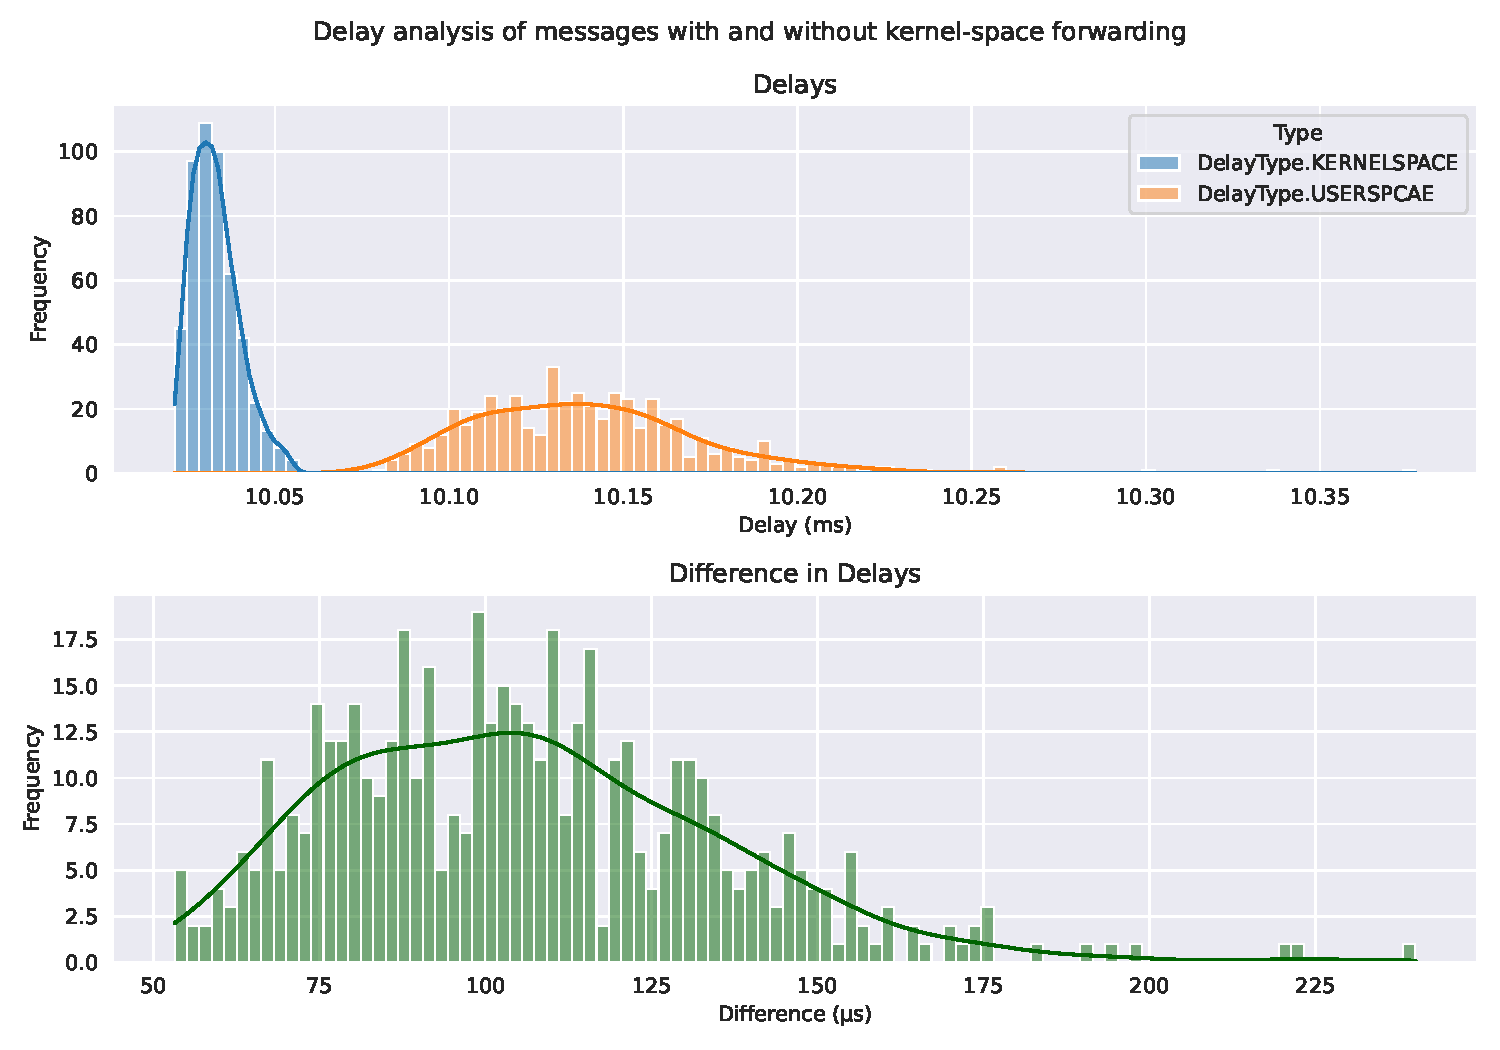
\includegraphics[width=\textwidth]{figures/04_testing_and_results/delays_small_packets_simple_userspace.pdf}
    \caption[Delay analysis of eBPF approach]{The blue and orange parts of the plot show the delay of a 
    kernel- and userspace-forwarded packet, respectively. Delay is measured as time passed between
    leaving the server eBPF program and entering the client eBPF program.
    The green part shows the raw difference between the delays of the same packet, which was sent via both 
    kernel- and userspace-forwarding.}\label{fig:delay-improvement}
\end{figure}
\vspace{0.5cm}

\subsection{CPU Utilization Comparison}
Besides showing that our approach reduces packet delay, we also measured that the CPU usage is 
not negatively impacted by our streaming system.
\autoref{fig:cpu-utilization-server},~\ref{fig:cpu-utilization-relay} and~\ref{fig:cpu-utilization-client}
show the CPU usage of the server, relay, and client processes, respectively, both with and without eBPF forwarding.
It is observable that none of the utilizations significantly differs between the two setups.
We created these CPU measurements by accumulating the CPU usage of all processes that are related 
to the respective parts of the setup.
The tag \verb|user| identifies the traditional setup where packets go all the way up to userspace while 
\verb|kernel| identifies the setup where packets are forwarded directly from within the kernel.

\begin{figure}[H]
    \begin{minipage}{0.48\textwidth}
        \centering
        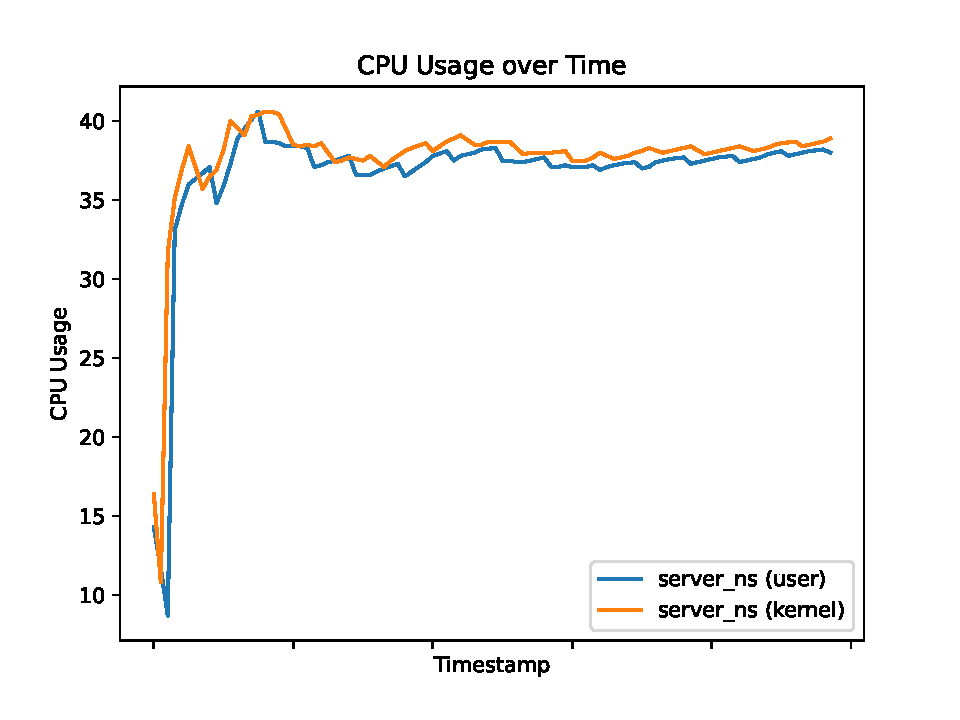
\includegraphics[width=1\linewidth]{figures/04_testing_and_results/cpu_usage_server_ns.pdf}
        \caption[Server CPU usage comparison]{Accumulated server CPU usage comparison.}\label{fig:cpu-utilization-server}
    \end{minipage}\hfill
    \begin{minipage}{0.48\textwidth}
        \centering
        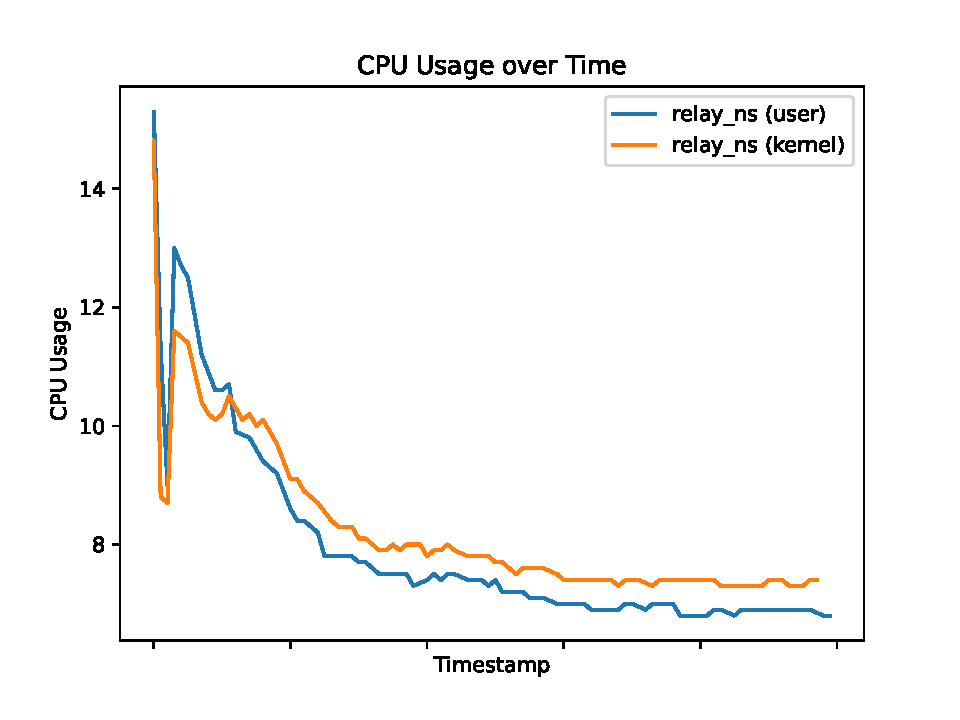
\includegraphics[width=1\linewidth]{figures/04_testing_and_results/cpu_usage_relay_ns.pdf}
        \caption[Relay CPU usage comparison]{Accumulated relay CPU usage comparison.}\label{fig:cpu-utilization-relay}
    \end{minipage}\hfill
    \begin{minipage}{\textwidth}
        \centering
        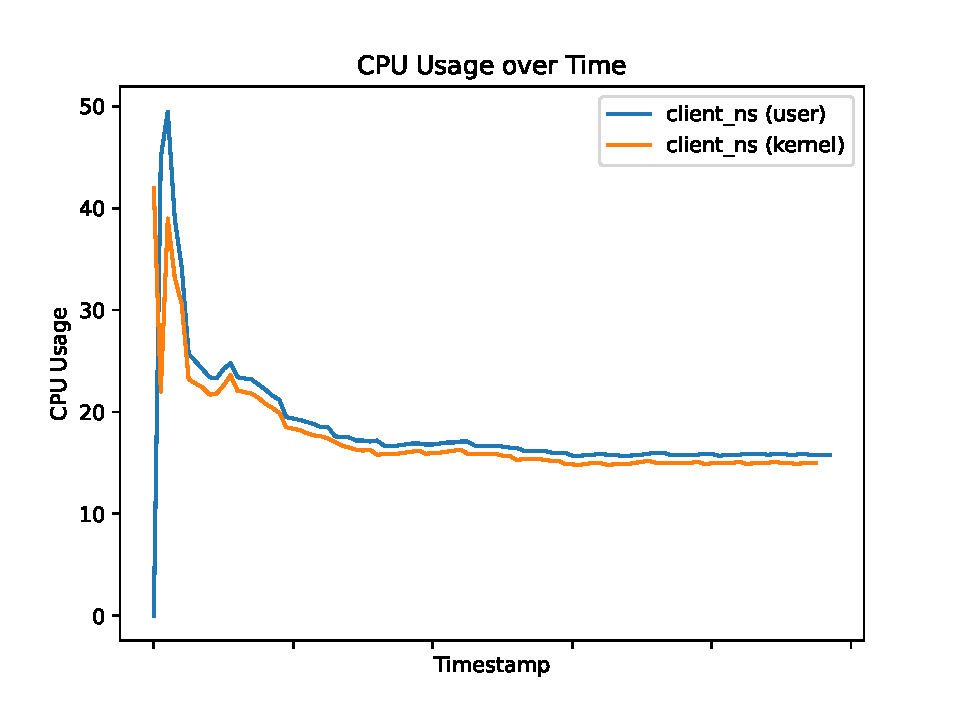
\includegraphics[width=0.48\textwidth]{figures/04_testing_and_results/cpu_usage_client_ns.pdf}
        \caption[Client CPU usage comparison]{Accumulated client CPU usage comparison.}\label{fig:cpu-utilization-client}
    \end{minipage}
\end{figure}

% TODO: remove?
% We also looked more closely which parts of our system take up the most CPU time and compared them
% to the most CPU-intensive parts of the initial userspace forwarding.
% \autoref{tab:cpu-usage-top} shows the top 10 functions that take up the most CPU time in our newly
% developed setup while~\autoref{tab:non-ebpf-cpu-usage-top} shows the same for the old userspace 
% forwarding setup without any eBPF interference. % TODO: make sure reference labels are correct
% We can clearly see that our setup is executing a lot of system calls which is to be expected
% due to the ongoing communication between the userspace and the kernel (i.e.~eBPF maps).
% TODO: measure non ebpf table and compare specific differences 

% \begin{table}
\caption{Table for CPU usage of relay Go processes}
\label{tab:cpu-usage-top}
\begin{tabular}{llllll}
\toprule
flat & flat\% & sum\% & cum & cum\% & cause \\
\midrule
440ms & 28.39\% & 28.39\% & 440ms & 28.39\% & runtime/internal/syscall.Syscall6 \\
140ms & 9.03\% & 37.42\% & 140ms & 9.03\% & runtime.futex \\
120ms & 7.74\% & 45.16\% & 120ms & 7.74\% & runtime.cgocall \\
40ms & 2.58\% & 47.74\% & 40ms & 2.58\% & runtime.write1 \\
30ms & 1.94\% & 49.68\% & 60ms & 3.87\% & runtime.checkTimers \\
30ms & 1.94\% & 51.61\% & 50ms & 3.23\% & runtime.mapaccess2 \\
20ms & 1.29\% & 52.90\% & 70ms & 4.52\% & .../cilium/ebpf/internal/unix.Syscall \\
20ms & 1.29\% & 54.19\% & 20ms & 1.29\% & net.IP.String \\
20ms & 1.29\% & 55.48\% & 20ms & 1.29\% & runtime.casgstatus \\
20ms & 1.29\% & 56.77\% & 20ms & 1.29\% & runtime.duffcopy \\
\bottomrule
\end{tabular}
\end{table}
 % TODO: also include table for "normal" relay and compare difference in what functions use most CPU 
% % \begin{table}
\caption{Table for cumulative CPU usage of relay Go processes}
\label{tab:example}
\begin{tabular}{llllll}
\toprule
flat & flat\% & sum\% & cum & cum\% & cause \\
\midrule
0.44s & 28.39\% & 28.39\% & 0.44s & 28.39\% & runtime/internal/syscall.Syscall6 \\
0 & 0\% & 28.39\% & 0.43s & 27.74\% & runtime.mcall \\
0.01s & 0.65\% & 29.03\% & 0.42s & 27.10\% & runtime.schedule \\
0 & 0\% & 29.03\% & 0.41s & 26.45\% & runtime.park\_m \\
0 & 0\% & 29.03\% & 0.40s & 25.81\% & syscall.RawSyscall6 \\
0.01s & 0.65\% & 29.68\% & 0.32s & 20.65\% & runtime.findRunnable \\
0 & 0\% & 29.68\% & 0.28s & 18.06\% & .../quic-go-prio-packs.(*connection).run \\
0 & 0\% & 29.68\% & 0.28s & 18.06\% & syscall.Syscall \\
0 & 0\% & 29.68\% & 0.23s & 14.84\% & .../quic-go-prio-packs.(*Transport).listen \\
0 & 0\% & 29.68\% & 0.23s & 14.84\% & .../quic-go-prio-packs.(*connection).run.func2 \\
\bottomrule
\end{tabular}
\end{table}
 % TODO: this is kinda useless since it only shows the "wrapping" functions. Maybe remove?
% \begin{table}
    \caption{Table for cumulative CPU usage of relay Go processes without fast-relays enabled.}
    \label{tab:non-ebpf-cpu-usage-top}
    \begin{tabular}{llllll}
    \toprule
    flat & flat\% & sum\% & cum & cum\% & cause \\
    \midrule
    TODO & TODO & TODO & TODO & TODO & TODO \\
    \bottomrule
\end{tabular}
\end{table}
     % TODO: actually measure

\hyperref[chap:appendix-fast-relay]{Appendix A} and~\hyperref[chap:appendix-plain-relay]{B} show 
the syscall usage of a 30-second video streaming example considering a setup with and without eBPF 
forwarding, respectively.
We trace this using\textit{strace} while considering the main process as well as all child processes
it creates and interacts with.
When comparing the two tables, one can see that our approach uses significantly fewer system calls.
This is partially due to a reduced need for userspace synchronization, decreasing the number of \verb|futex| syscalls.
Other syscalls like \verb|epoll_pwait| or \verb|nanosleep| are also used significantly less.

The concrete impact of our setup on system calls can be seen at the bottom 
of~\hyperref[chap:appendix-fast-relay]{Appendix A} and~\hyperref[chap:appendix-plain-relay]{B} 
where total syscall counts are shown.
The setup using eBPF forwarding uses 225674 during our example transmission, while the traditional setup 
uses 296132 syscalls.
This means our setup uses roughly 24\% fewer syscalls than the traditional one.
Regarding \verb|futex| calls, our setup uses a little more than 34\% 
fewer than the traditional setup, with 21666 calls instead of 32940.
Even bigger percentage differences can be seen for \verb|nanosleep| calls with a reduction of 
approximately 42\% (14293 instead of 24716) and \verb|epoll_pwait| calls with 
an improvement of around 67\% (11289 instead of 34149).

Another observation we made was that the eBPF setup uses fewer \verb|bpf| syscalls than we would have assumed for 
the amount of traffic that happened in the test.
This might be caused by optimizations happening in the eBPF library used by our Go application.
Such optimizations might include reducing the number of \verb|bpf| syscalls 
by combining multiple map reads into one syscall.
We did, however, not investigate how this underlying library works and how our 
eBPF communication could be optimized further.
\section{Summary}\label{sec:summary_ch4}

We have presented the results of comparing our newly developed 
relay design to a traditional relay system without eBPF usage.
We were able to show that the idea of delaying any non-essential
application-layer processing until after the packet was forwarded
does provide a performance benefit, while utilizing a similar 
amount of CPU resources.
The fact that our system works also shows that eBPF is capable of 
providing basic relay functionality despite possible limitations
due to its verifier.
In the following chapter, we will conclude our work and provide
an outlook on future work that can be done in this area.